\documentclass{beamer}

%
% Choose how your presentation looks.
%
% For more themes, color themes and font themes, see:
% http://deic.uab.es/~iblanes/beamer_gallery/index_by_theme.html
%
\mode<presentation>
{
  \usetheme{default}      % or try Darmstadt, Madrid, Warsaw, ...
  \usecolortheme{default} % or try albatross, beaver, crane, ...
  \usefonttheme{default}  % or try serif, structurebold, ...
  \setbeamertemplate{navigation symbols}{}
  \setbeamertemplate{caption}[numbered]
  \setbeamertemplate{footline}[page number]
  \setbeamercolor{frametitle}{fg=white}
  \setbeamercolor{footline}{fg=black}
} 

\usepackage[english]{babel}
\usepackage[utf8x]{inputenc}
\usepackage{tikz}
\usepackage{listings}
\usepackage{courier}

\xdefinecolor{darkblue}{rgb}{0.1,0.1,0.7}
\xdefinecolor{dianablue}{rgb}{0.18,0.24,0.31}
\definecolor{commentgreen}{rgb}{0,0.6,0}
\definecolor{stringmauve}{rgb}{0.58,0,0.82}

\lstset{ %
  backgroundcolor=\color{white},      % choose the background color
  basicstyle=\ttfamily\small,         % size of fonts used for the code
  breaklines=true,                    % automatic line breaking only at whitespace
  captionpos=b,                       % sets the caption-position to bottom
  commentstyle=\color{commentgreen},  % comment style
  escapeinside={\%*}{*)},             % if you want to add LaTeX within your code
  keywordstyle=\color{blue},          % keyword style
  stringstyle=\color{stringmauve},    % string literal style
  showstringspaces=false,
  showlines=true
}

\lstdefinelanguage{scala}{
  morekeywords={abstract,case,catch,class,def,%
    do,else,extends,false,final,finally,%
    for,if,implicit,import,match,mixin,%
    new,null,object,override,package,%
    private,protected,requires,return,sealed,%
    super,this,throw,trait,true,try,%
    type,val,var,while,with,yield},
  otherkeywords={=>,<-,<\%,<:,>:,\#,@},
  sensitive=true,
  morecomment=[l]{//},
  morecomment=[n]{/*}{*/},
  morestring=[b]",
  morestring=[b]',
  morestring=[b]"""
}

\title[2016-06-13-high-level-low-level]{High-level analysis scripts \\ with low-level performance}
\author{Jim Pivarski}
\institute{Princeton University -- DIANA}
\date{June 13, 2016}

\begin{document}

\logo{\pgfputat{\pgfxy(0.11, 8)}{\pgfbox[right,base]{\tikz{\filldraw[fill=dianablue, draw=none] (0 cm, 0 cm) rectangle (50 cm, 1 cm);}}}\pgfputat{\pgfxy(0.11, -0.6)}{\pgfbox[right,base]{\tikz{\filldraw[fill=dianablue, draw=none] (0 cm, 0 cm) rectangle (50 cm, 1 cm);}
\includegraphics[height=0.99 cm]{diana-hep-logo.png}\tikz{\filldraw[fill=dianablue, draw=none] (0 cm, 0 cm) rectangle (4.9 cm, 1 cm);}}}}

\begin{frame}
  \titlepage
\end{frame}

\logo{\pgfputat{\pgfxy(0.11, 8)}{\pgfbox[right,base]{\tikz{\filldraw[fill=dianablue, draw=none] (0 cm, 0 cm) rectangle (50 cm, 1 cm);}
\includegraphics[height=1 cm]{diana-hep-logo.png}}}}

% Uncomment these lines for an automatically generated outline.
%\begin{frame}{Outline}
%  \tableofcontents
%\end{frame}

\begin{frame}{}
\vfill
This talk is about a future project I'm working toward.

\vfill
\begin{block}{Goals:}
\begin{itemize}
\item to increase the separation between physics-relevant concepts and low-level computing details
\item without sacrificing computational performance; in most cases, improving it.
\end{itemize}
\end{block}
\end{frame}

\begin{frame}{}
\vfill
This talk is about programming languages because languages {\it are the user interface} of data analysis.

\vfill
The same is true in industry:
\begin{itemize}
\item business intelligence speaks SQL,
\item statisticians speak R and SAS,
\item financial analysts write extensive Excel macros\ldots
\end{itemize}
\end{frame}

\begin{frame}{The choice of language matters}

\vspace{0.5 cm}
\begin{columns}
\column{0.7\linewidth}
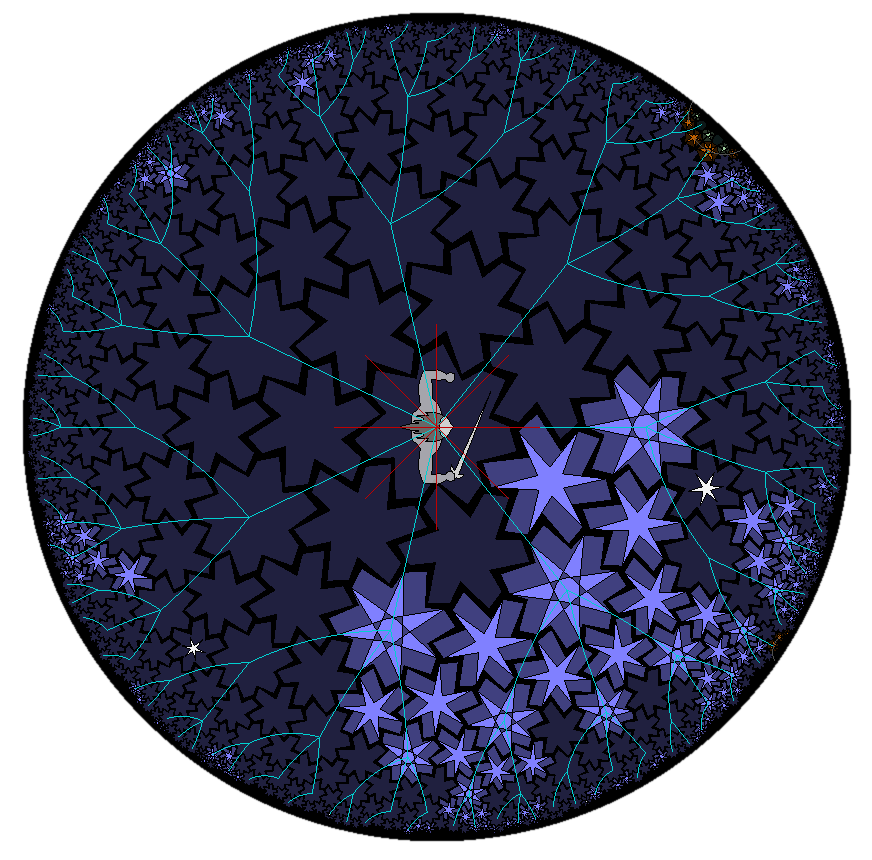
\includegraphics[width=\linewidth]{space-of-programs.png}

\column{0.3\linewidth}
All programming languages fill the ``space of possible programs'' because they're Turing complete.

\vspace{0.25 cm}
However, different languages are like different metrics on this space.

\vspace{0.25 cm}
A small change in one is a big change in another.
\end{columns}
\end{frame}

\begin{frame}{Evolution of language choice}
\vspace{0.5 cm}
\begin{block}{High energy physics}
Decades of Fortran, transitioned to C++ in late '90s, may be leaning towards Python now.
\end{block}

\begin{block}{Data science in industry}
Big Data/Hadoop grew out of web development: distributed systems in Java.

\vspace{0.25 cm}
Now involves more machine learning and statistics, so shift toward Scala on the JVM, Python for Scikit-Learn, and R.
\end{block}

\vspace{0.5 cm}
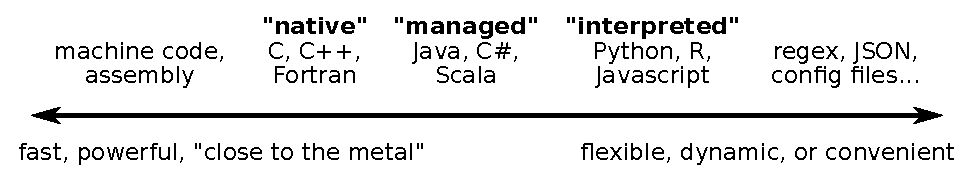
\includegraphics[width=\linewidth]{languages1.pdf}
\end{frame}

\begin{frame}{Abstractions {\it versus} performance?}
\vspace{0.5 cm}
Experience tells us that low-level is fast and high-level is slow.

\vspace{0.5 cm}
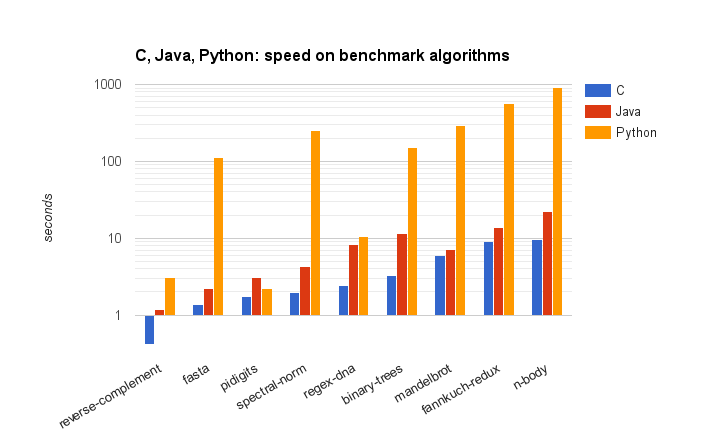
\includegraphics[width=\linewidth]{benchmark-games.png}

\hfill \textcolor{blue}{\small \url{http://benchmarksgame.alioth.debian.org/}}
\end{frame}

\begin{frame}{Domain-Specific Languages (DSLs)}

\vspace{0.5 cm}
\begin{columns}
\column{0.7\linewidth}
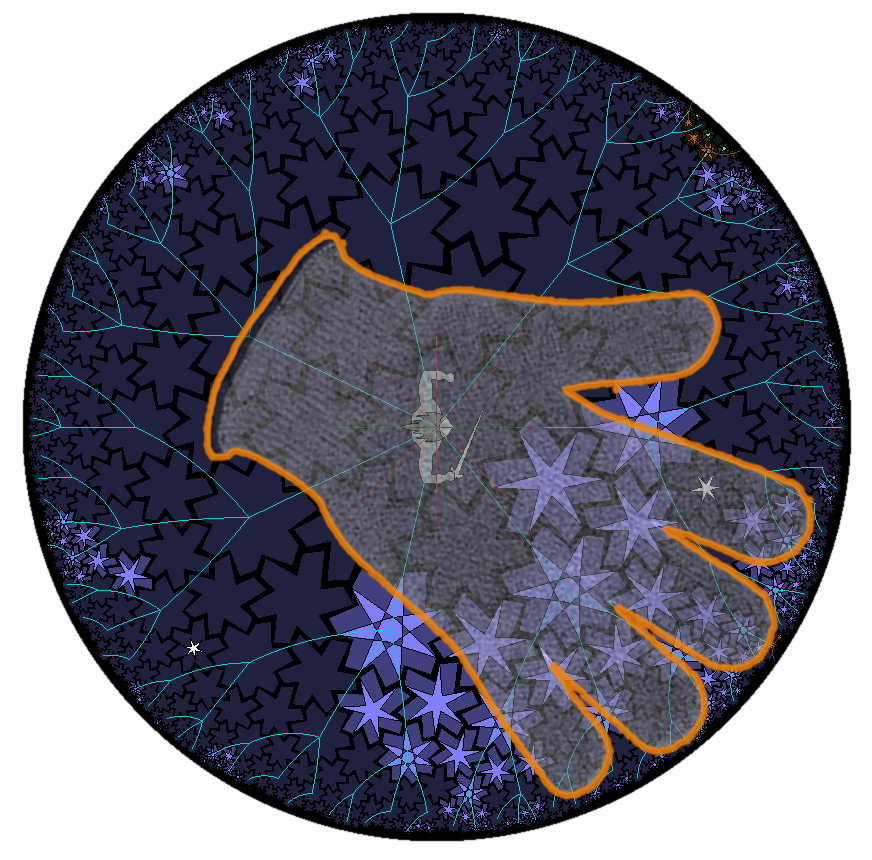
\includegraphics[width=\linewidth]{space-of-programs-glove.png}

\column{0.4\linewidth}
But it doesn't have to be: intentionally restricting the scope of the language allows more optimization.

\vspace{0.25 cm}
\textcolor{darkblue}{Prime example: SQL.}

\vspace{0.25 cm}
But also:
\begin{itemize}
\item Fortran's lack of (aliasable) pointers
\item regular expressions for string manipulation
\item Numpy in Python
\item Histogrammar\ldots
\end{itemize}
\end{columns}
\end{frame}

\begin{frame}{More accurate statement}

\vfill
High-level abstractions $+$ complete generality is slow.

\vfill
High-level abstractions $+$ restricted domain
\begin{itemize}
\item can be as fast as a custom-tuned program \mbox{(especially with JIT),\hspace{-1 cm}}
\item but with better separation of domain knowledge from computing details.
\end{itemize}

\vfill
\begin{uncoverenv}<2>
A well-designed DSL can encourage exploration of the problem space (physics) while the backend optimizes performance.

\vspace{0.25 cm}
(A poorly designed DSL can make it impossible to get work done!)
\end{uncoverenv}
\end{frame}

\begin{frame}{Goals for my future project}
\vfill
I plan to design a domain specific language for end-user physics analysis scripts with the following properties:

\begin{itemize}
\item a subset of or based on Python syntax
\item non-exclusive: mix with normal (slow) Python
\item immutable, maybe total-functional (next slide)
\item very strongly typed, but only through inference (next$^2$ slide)
\item manual optimizations via CSS-style selectors (next$^3$ slide)
\item supporting imperative idioms through patterns (next$^4$ slide)
\end{itemize}

\vfill
\uncover<2->{\textcolor{darkblue}{Scope:} only the data manipulation, not whole applications}

\vspace{0.1 cm}
\uncover<3->{\textcolor{darkblue}{Backends:} convert to C, CUDA/OpenCL, or Verilog/HDL for a traditional compiler to compile (``{\it transpiling} to C'')}

\vspace{0.1 cm}
\uncover<4->{\textcolor{darkblue}{Stepping stone:} Histogrammar, my histogram-aggregation DSL, is being used to test some of the basic ideas.}
\end{frame}

\begin{frame}{Immutable, maybe total-functional}
\vfill
``Functional programming'' eliminates mutable program state:
\begin{itemize}
\item output of functions depend strictly on their inputs
\item {\tt \small x = x + 1} is a false mathematical statement
\item assignments form a time-independent graph, may be written in any order and backend may execute in any order
\item backend may substitute mutable data structures by analyzing (or temporally rearranging) the assignment graph
\item good for concurrency (no locks)
\end{itemize}

\vfill
\begin{uncoverenv}<2->
``Total functional programming'' also eliminates unbounded loops and exceptions:
\begin{itemize}
\item programs are known to halt (not Turing complete), maybe even with time estimates from static analysis
\item exactly model mathematical functions: $f: \mathcal{D} \to \mathcal{R}$
\end{itemize}
\end{uncoverenv}
\end{frame}

\begin{frame}[fragile]{Strongly typed through inference}
\vfill
Type check is a formal proof that program is free of certain errors.

\vfill
Scala example (eliminates runtime null pointer exceptions):
\begin{lstlisting}[language=scala]
val numberOrNone: Option[Double] = Some(3.14)
val cosx = numberOrNone match {
  case Some(x) => cos(x)
  case None => -999.0
}

// or better
val cosxOrNone = numberOrNone.map(cos(_))

// but cos(numberOrNone) would be a compiler error
\end{lstlisting}
\end{frame}

\begin{frame}{Strongly typed through inference}
\vspace{0.3 cm}
\begin{itemize}
\item<1-> {\tt \small numberOrNone} is a value from the set $\mathbb{R} \cup \{\mbox{\tt \small None}\}$.

\item<2-> One could catch division-by-zero errors in the same way by considering sets like $\mathbb{R} \cup \{-\infty, \infty\}$.

\item<3-> For physics applications, it could be useful to consider any interval, like $[-3, 8] \cap \mathbb{Z}$ or $[0, \infty)$, as ``data types.''
\begin{itemize}
\item<4-> This is like an extreme form of {\tt \small int} versus {\tt \small unsigned int}.
\item<4-> Useful feedback to the data analyst: ``Why does my function output have such a large range?''
\item<4-> Could even be used to set bit widths for an FPGA backend.
\item<4-> I have implemented this for $+$, $-$, $*$, $/$, $**$, and modular arithmetic with 6k lines of unit tests. Extending to continuous functions will involve searches for inflection points.
\end{itemize}
\item<5-> Inference only: intervals specified on input arguments, everything else inferred. The compiler should be telling the user what the domains are, not the other way around. (Being purely functional helps this.)
\end{itemize}
\end{frame}

\begin{frame}{Optimizations via CSS-style selectors}
\vfill
High-level code is frustrating when it {\it takes away} the ability to manually optimize.

\vfill
The point is not to make the physicist unaware of the low-level details, just to remove the necessity of thinking about both at the same time.

\vfill
\uncover<2>{(You don't have to think about nuclear physics when studying atomic structure, but that doesn't mean you can't {\it know about} nuclear physics!)}
\end{frame}

\begin{frame}[fragile]{Optimizations via CSS-style selectors}
\vfill
Take a hint from HTML+CSS, which separates structure from style by putting them in two separate files:

\vspace{0.25 cm}
\begin{columns}[T]
\column{0.55\linewidth}
{\bf \small HTML file}

\begin{lstlisting}[language=html, basicstyle=\ttfamily\scriptsize]
<html>
  <body>
    <ul id="bulleted-list">
      <li class="first">one</li>
      <li class="rest">two</li>
      <li class="rest">three</li>
    </ul>
    <ol>
      <li>unaffected</li>
    </ol>
  </body>
</html>
\end{lstlisting}

\column{0.4\linewidth}
{\bf \small CSS file}

\begin{lstlisting}[basicstyle=\ttfamily\scriptsize]
#id { border: solid 1px red; }

ul li { color: blue; }

li.first { font-weight: bold; }

.rest { text-decoration: underline; }
\end{lstlisting}
\end{columns}
\end{frame}

\begin{frame}[fragile]{Optimizations via CSS-style selectors}
\vfill
Consider a variant of CSS selectors that picks program elements and applies optimization hints:

\vspace{0.25 cm}
\begin{columns}[T]
\column{0.5\linewidth}
{\bf \small Correctness}

\begin{lstlisting}[language=python, basicstyle=\ttfamily\scriptsize]
# type declarations as Python3 argument decorations
def doWeirdStuff(
      x: [-10, 10],
      xs: list(size=[1, inf],
               data=[-5, 5])):

    # function body
    xs2 = xs.appended(xs[0])

    return xs2.appended(x / 2)
\end{lstlisting}

\column{0.55\linewidth}
{\bf \small Performance}

\begin{lstlisting}[language=c, basicstyle=\ttfamily\scriptsize]
/* only affects x in doWeirdStuff, not other functions */
doWeirdStuff x {
  data-type: signed char;
}

/* implies that xs2 is also a mutable linked list */
xs {
  data-type: mutable linked list;
  storage: contiguous obstack;
}
\end{lstlisting}
\end{columns}

\vfill
\hfill \textcolor{gray}{Status: not deeply thought-through yet.}
\end{frame}

\begin{frame}{Imperative idioms through patterns}
\begin{block}{Problem with Python}
Large-scale syntax isn't suited for functional programming:
\begin{itemize}
\item control in statements, not expressions
\item cannot put statements in lambda functions
\end{itemize}
\end{block}

\vspace{0.25 cm}
\begin{block}{Problem with anything else}
Unfamiliar to physicists: yet another language!

\vspace{0.3 cm}
Besides, Python's expression syntax is excellent, want to keep that.
\end{block}
\end{frame}

\begin{frame}[fragile]{Imperative idioms through patterns}
\only<2>{\vfill\vfill}
\vfill
\begin{columns}
\column{0.5\linewidth}
Imperative code, the way Python was meant to be used:

\begin{lstlisting}[language=python, basicstyle=\ttfamily\scriptsize]
def function(x: (-inf, inf)):
    if x > 0:
        y = 1
    elif x < 0:
        y = -1
    else:
        y = 0

    tenOfThem = []
    for i in range(10):
        tenOfThem.append(y)
    return tenOfThem
\end{lstlisting}

\column{0.5\linewidth}
Functional code, the way I'd want to use it:

\begin{lstlisting}[language=python, basicstyle=\ttfamily\scriptsize]
def function(x: (-inf, inf)):
    y =  1 if x > 0 else
        -1 if x < 0 else
         0

    tenOfThem = range(10) \
        .map(lambda i: y)

    return tenOfThem



\end{lstlisting}
\end{columns}

\vfill
\begin{onlyenv}<1>
I have to think backwards to read the one on the right.
\end{onlyenv}
\begin{onlyenv}<2>
But suppose the left is recognized as ``idioms'' and translated?
\begin{itemize}
\item {\tt \small if} statements where every branch defines the same symbol
\item {\tt \small for} loops that only append to a list
\end{itemize}
\end{onlyenv}
\end{frame}

\begin{frame}[fragile]{Transpiling in Histogrammar}
\vfill
Histogrammar is a DSL with a much smaller scope (making histograms in distributed systems).

\vfill
Deeply nested structure is a nice abstraction, but it's surely slower than filling an array.

\begin{lstlisting}[language=python, basicstyle=\ttfamily\scriptsize]
directory_of_histograms =
    Label(
        one = Select(lambda d: d.trigger > 5,
                  Bin(100, 0, 80, lambda d: d.pt, Count())),
        two = Select(lambda d: d.pt > 30,
                  Bin(100, 0, 120, lambda d: d.met, Count()))
    )
\end{lstlisting}

\vfill
\begin{uncoverenv}<2->
{\bf Transparent speed-up: JIT compilation}

\textcolor{blue}{\small \url{http://github.com/diana-hep/histogrammar/scala-jit}}

transpiles the histogram structure into explicit C code, compiles it, and runs it.
\end{uncoverenv}
\end{frame}

\begin{frame}[fragile]{Transpiling in Histogrammar}
\vspace{0.3 cm}
Auto-generated C code operates on batches of data, batches of histograms, by casting pointers in a contiguous malloc block.

\vfill
\begin{lstlisting}[language=c, basicstyle=\ttfamily\tiny]
#include <inttypes.h>
#include <math.h>

uint64_t loop(void *dataBatch, void *storageBatch, int32_t inputBufferFill) {
  uint64_t storagePointer;
  uint64_t BinningUnwind_0;
  double BinningQuantity_0;
  int32_t BinningBin_0;
  for (int32_t rowIndex = 0;  rowIndex < inputBufferFill;  ++rowIndex) {
    storagePointer = (uint64_t)storageBatch;
    // Binning unwind-protect
    BinningUnwind_0 = storagePointer;
    BinningQuantity_0 = (*((double*)(dataBatch + 0 + rowIndex*8)));
    if (BinningQuantity_0 != BinningQuantity_0) {
      // Binning.nanflow
      storagePointer += 816;
      // Counting.entries without weight
      ++(*((int32_t*)storagePointer));
      storagePointer += 8;
    }
    else {
      BinningBin_0 = (int32_t)floor(100 * (BinningQuantity_0 - 0.0) * 0.0125);
      if (BinningQuantity_0 == -INFINITY  ||  BinningBin_0 < 0) {
        // Binning.underflow
        storagePointer += 800;
        // Counting.entries without weight
        ++(*((int32_t*)storagePointer));
\end{lstlisting}
\end{frame}

\begin{frame}{Transpiling in Histogrammar}
\renewcommand{\arraystretch}{1.2}
\vfill
\vfill
The whole workflow (calculating data in Scala, copying to off-heap, filling histograms, bringing back results):

\begin{center}
\begin{tabular}{r r c c}
\#histograms & \#entries & naive Scala & JIT C \\\hline
1 & 10,000,000 & 13 seconds & 0.81 seconds \\
100 & 100,000 & 27 seconds & 0.75 seconds \\
\end{tabular}
\end{center}

\vfill
Just the tight loop around filling (pull data from an array) and using cling instead of tcc:

\begin{center}
\begin{tabular}{r r c c}
\#histograms & \#entries & JIT C & ROOT \\\hline
1 & 100,000,000 & 0.74 seconds & 2.2 seconds \\
100 & 1,000,000 & 0.44 seconds & 2.2 seconds \\
\end{tabular}
\end{center}
\end{frame}

\begin{frame}{Prior art: tools to use \& interoperate with}
\begin{onlyenv}<1>
\vspace{0.75 cm}
\textcolor{darkblue}{\Large Cython:} adds performance hints to Python so that it can be more easily compiled into extension modules (C code for gcc).

\begin{center}
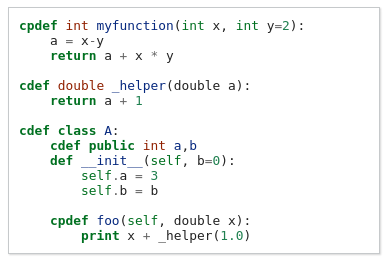
\includegraphics[width=0.8\linewidth]{cython.png}
\end{center}
\end{onlyenv}
\begin{onlyenv}<2>
\vspace{0.5 cm}
\textcolor{darkblue}{\Large Numba:} propagates Numpy types through a Python function to produce LLVM bytecode for JIT compilation.

\vspace{0.2 cm}
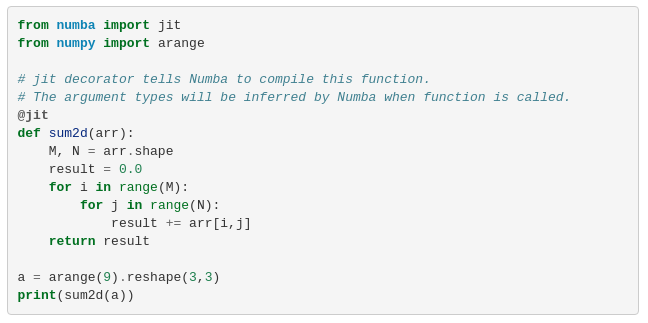
\includegraphics[width=\linewidth]{numba.png}
\end{onlyenv}
\begin{onlyenv}<3>
\vspace{0.5 cm}
\textcolor{darkblue}{\Large SymPy:} symbolic algebra system in Python (expression graph is a functional program, which can be simplified).

\vspace{0.2 cm}
\textcolor{darkblue}{\Large Theano:} matrix expression compiler with CPUs and GPUs.

\vspace{0.2 cm}
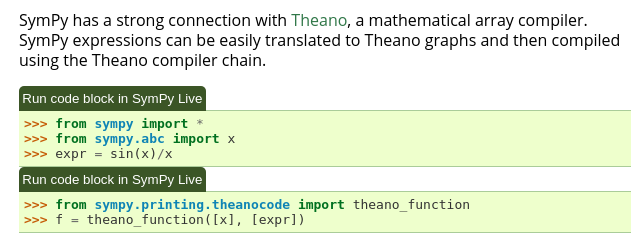
\includegraphics[width=\linewidth]{sympy_theano.png}
\end{onlyenv}

\begin{onlyenv}<4>
\vspace{0.5 cm}
\textcolor{darkblue}{\Large PyCUDA/PyOpenCL:} dispatches kernels to GPU.

\vspace{0.2 cm}
\textcolor{darkblue}{\Large CodePy:} AST for CUDA/OpenCL (same author).

\begin{center}
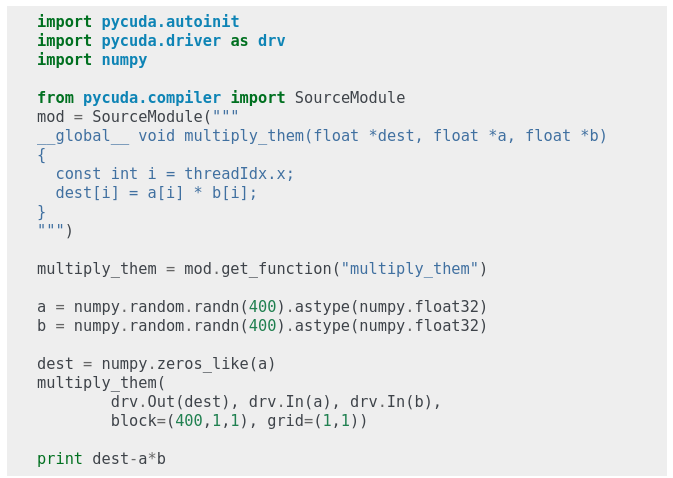
\includegraphics[width=0.8\linewidth]{pycuda_pyopencl_codepy.png}
\end{center}
\end{onlyenv}
\end{frame}

\begin{frame}{Recap}
High-level abstractions are not inconsistent with computational performance when the problem domain is sufficiently restricted.

\vfill
I'm planning to expand my current work from histogramming abstractions to a domain specific language for physics analysis \mbox{that is:}
\begin{itemize}
\item familiar enough to be used by physicists
\item designed around the specific needs of physics analysis
\item transpiled to highly performant code.
\end{itemize}
\end{frame}

\begin{frame}{Greg Owen's talk on JIT in Spark 2.0}
\vspace{1 cm}
\only<1>{
\includegraphics[width=\linewidth]{greg-owen/page1.png}}
\only<2>{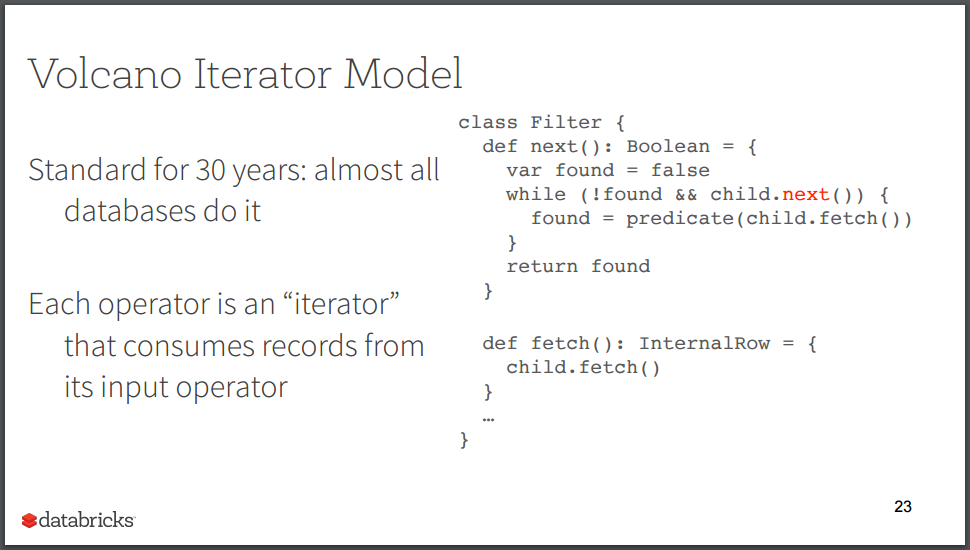
\includegraphics[width=\linewidth]{greg-owen/page2.png}}
\only<3>{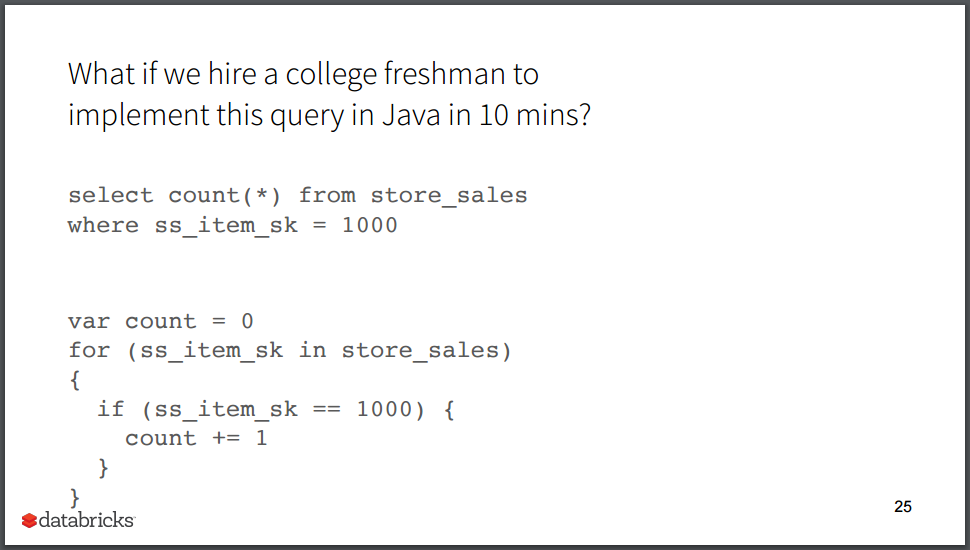
\includegraphics[width=\linewidth]{greg-owen/page3.png}}
\only<4>{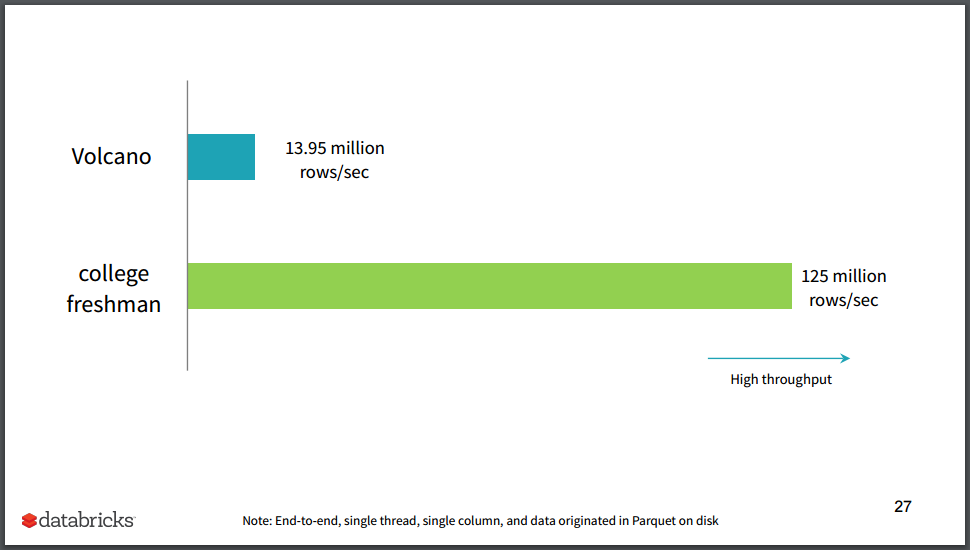
\includegraphics[width=\linewidth]{greg-owen/page4.png}}
\only<5>{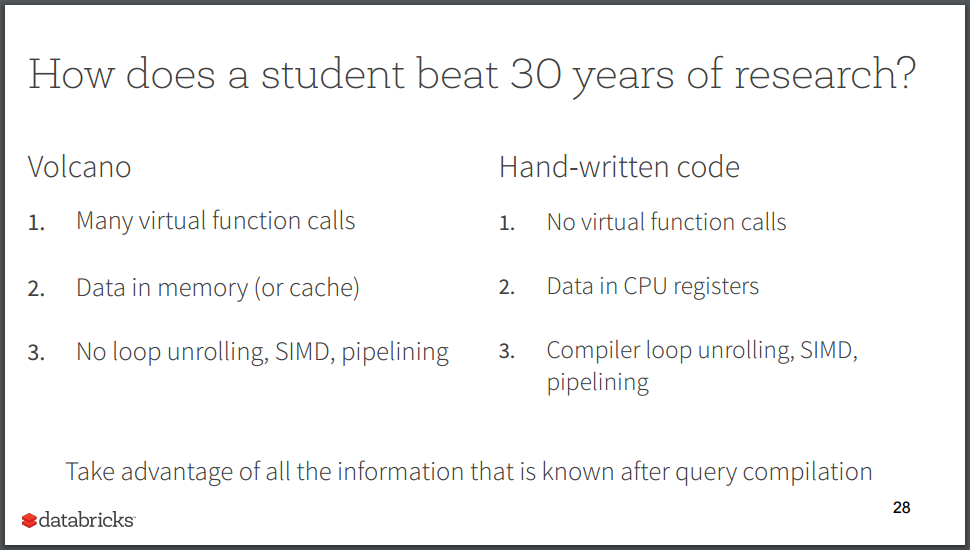
\includegraphics[width=\linewidth]{greg-owen/page5.png}}
\end{frame}
\end{document}
